\documentclass[a4paper,11pt]{style-esi/td}

\usepackage{style-esi/licence}	% Affiche une licence dans le document
\usepackage{style-esi/exercice}
\usepackage{style-esi/listing}
\usepackage{style-esi/tutoriel}
\usepackage{style/dev1}
\marginnumbertrue

\newcommand{\image}[2]{{\par\centering \includegraphics[height=#2]{image/#1}\par}
}
\begin{document}

\seancesimple{X}{Une introduction à Git sous NetBeans}

\bigskip
\begin{abstract}
	\noindent
	Un logiciel de gestion de versions comme \bsc{git} permet notamment de :
	\begin{itemize}
	\item 
		gérer l'historique d'un projet en sauvant chaque version
		et la description de ce qu'elle apporte ;
	\item
		sauver le projet (dans toutes ses versions) sur un serveur ;
	\item 
		le retrouver facilement sur une autre machine.
	\end{itemize}
	Le but de ce TD est de vous offrir 
	une introduction à \bsc{git} en utilisant \bsc{Netbeans}.
	Un TD du laboratoire environnement vous permettra 
	d'apprendre à utiliser \bsc{git} en mode commande
	pour aller plus loin dans sa compréhension et son utilisation.
\end{abstract}

\bigskip
\tableofcontents
\newpage

%===================
\section{Utiliser \bsc{git} avec \bsc{Netbeans} en local}
%====================	

Explorons comment demander à \bsc{git} de suivre notre projet 
et comment créer et décrire ses différentes versions.

%\subsection{Création d'un projet dans Netbeans}
%==============================================

\begin{Tutoriel}{Créer un projet sous Netbeans}
%------------------------------------------------------------------
	Commençons par créer un projet que nous allons pouvoir faire suivre par \bsc{git}.
	\begin{steps}
	\item
		Créez un nouveau projet \bsc{NetBeans} appelé \samp{HelloGit}.
		Ce projet sera constitué  :
		\begin{itemize}
		\item 
			d'un package \samp{dev1.javl} ;
		\item
			d'une classe principale appelée \samp{HelloGit}
			qui affiche le numéro de version du projet.
		\end{itemize}
		\image{NetBeans_Project_01}{4cm}
	\item 
		Vous pouvez l'exécuter pour vérifier que tout va bien.
	\end{steps}
\end{Tutoriel}

\begin{Tutoriel}{Initialisation de l'historisation}
%------------------------------------------------------------------
	Nous allons maintenant demander à git de suivre \emph{localement} notre projet.
	Pour ce faire, suivez les étapes suivantes sous Netbeans :
	\begin{steps}
	\item
		Dans l'onglet \samp{Projects} (à gauche) 
		cliquez droit sur le projet \samp{TestGit}.
	\item 
		Choisissez l'option \samp{Versioning}.
	\item 
		Suivi de l'option \samp{Initialize Git Repository...}.
		\image{NetBeans_Push01}{6cm}
	\item 
		Un pop-up vous propose de choisir le dossier 
		qui contiendra l'historique local.
		Conservez le chemin proposé par défaut, 
		il s'agit du répertoire de votre projet.
	\end{steps}
\end{Tutoriel}

Remarquez que le nom du fichier \samp{HelloGit.java}
est à présent en vert.
\bsc{Git} utilise un code couleur pour indiquer l'état du fichier.
\begin{itemize}
\item 
	Le {\color{green!50!black} vert}
	indique qu'il s'agit d'un nouveau fichier qui n'a jamais 
	fait l'objet d'une sauvegarde dans \bsc{git}.
\item 
	Le {\color{blue} bleu}
	indiquera qu'il s'agit d'un fichier qui a été modifié
	depuis sa sauvegarde dans \bsc{git}.
\end{itemize}

\newpage
\begin{Tutoriel}{Un premier commit}
%------------------------------------------------------------------
	Imaginons que la première fonctionnalité de votre projet soit terminée : 
	vous savez afficher la version du projet dans la console.
	Comme cette partie du développement est clôturée, 
	vous souhaitez l'enregistrer dans l'historique du projet.

	\begin{infoit}{Commit}
		Un \textbf{commit} (ou \textbf{soumission} en français)
		contient l’ensemble des fichiers et leur contenu qui composaient
		le projet à un moment donné. 
		Il contient également une série d'informations
		comme une date de création, le nom du créateur et une description. 
	\end{infoit}

	Pour effectuer ce premier commit, suivez les étapes suivantes :
	\begin{steps}
	\item 
		Dans l'onglet \samp{Projects} cliquez droit sur le projet.
		\begin{alertbox}
			Attention ! 
			Une erreur courante est de cliquer droit sur un fichier et non sur le projet.
			Seules les modifications de ce fichier sont commitées dans ce cas, 
			ce qui n'est généralement pas l'action souhaitée.
		\end{alertbox}
	\item 
		Sélectionnez l'option \samp{Git} puis l'option \samp{Commit...}
		\image{NetBeans_Push02}{5cm}
	\end{steps}

	Cette action vous renvoie vers l'écran de validation des \emph{commits}
	où vous pourrez décrire ce que vous venez de développer.
	\image{NetBeans_Push03}{5cm}
	On y trouve également la liste tous les fichiers qui ont été créés,  
	modifiés ou supprimés par votre travail.
	Comme il s'agit d'un nouveau projet, 
	il s'agit ici des fichiers créés et gérés par \bsc{NetBeans}
	en plus de la classe \samp{HelloGit}.
	\begin{steps}
	\item 
		Écrivez le message suivant dans la partie \samp{Commit Message} :\\
		\samp{"Création du projet et affichage du numéro de version"}.
	 \item 
		Terminez l'opération en cliquant sur le bouton \samp{Commit}.
	\end{steps}
\end{Tutoriel}

\begin{Tutoriel}{Nouvelle fonctionnalité\dots{} Nouveau Commit}
%------------------------------------------------------------------
	Dans le cadre de ce projet une nouvelle fonctionnalité est demandée,
	l'utilisateur doit encoder son nom.
	\begin{steps}
	\item 
		Modifiez le programme afin qu'il demande le nom de l'utilisateur :
		\begin{center}
			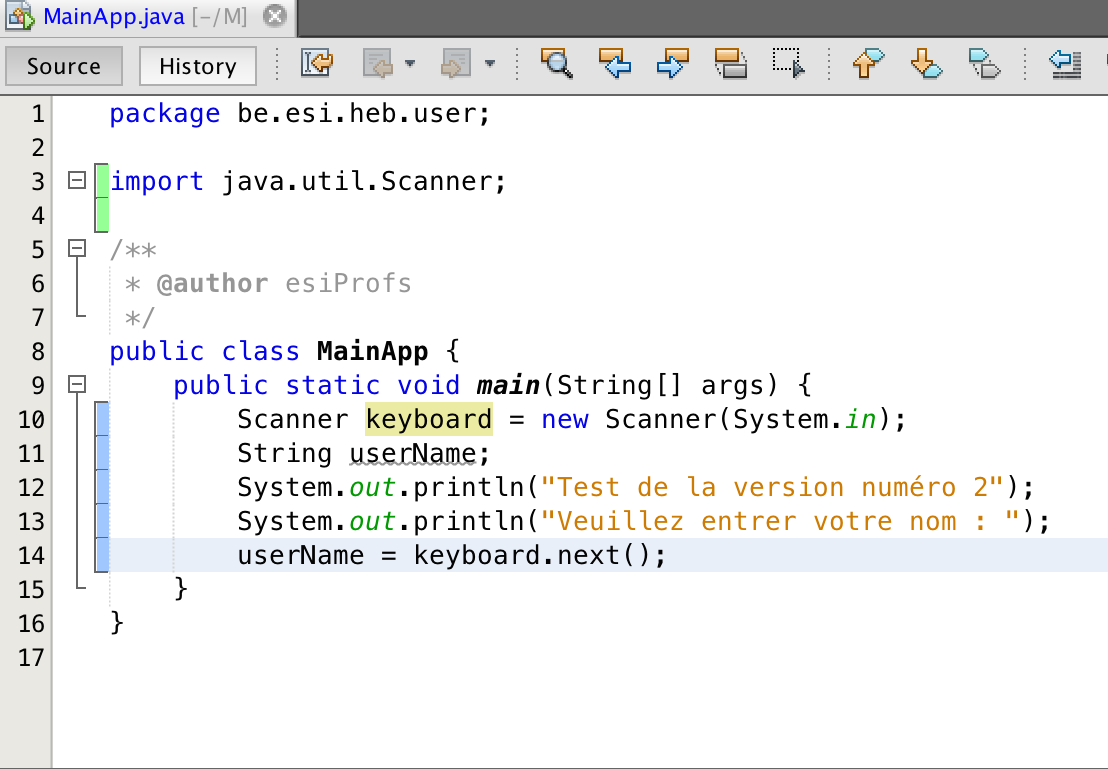
\includegraphics[width=.7\textwidth]{image/NetBeans_Project_03.png}
		\end{center}
	\end{steps}
	Afin de conserver dans l'historique cette nouvelle version du projet, 
	il faut effectuer un nouveau \emph{commit}.
	\begin{steps}
	\item 
		Effectuez ce commit comme expliqué dans le tutorial précédent.
		\begin{center}
			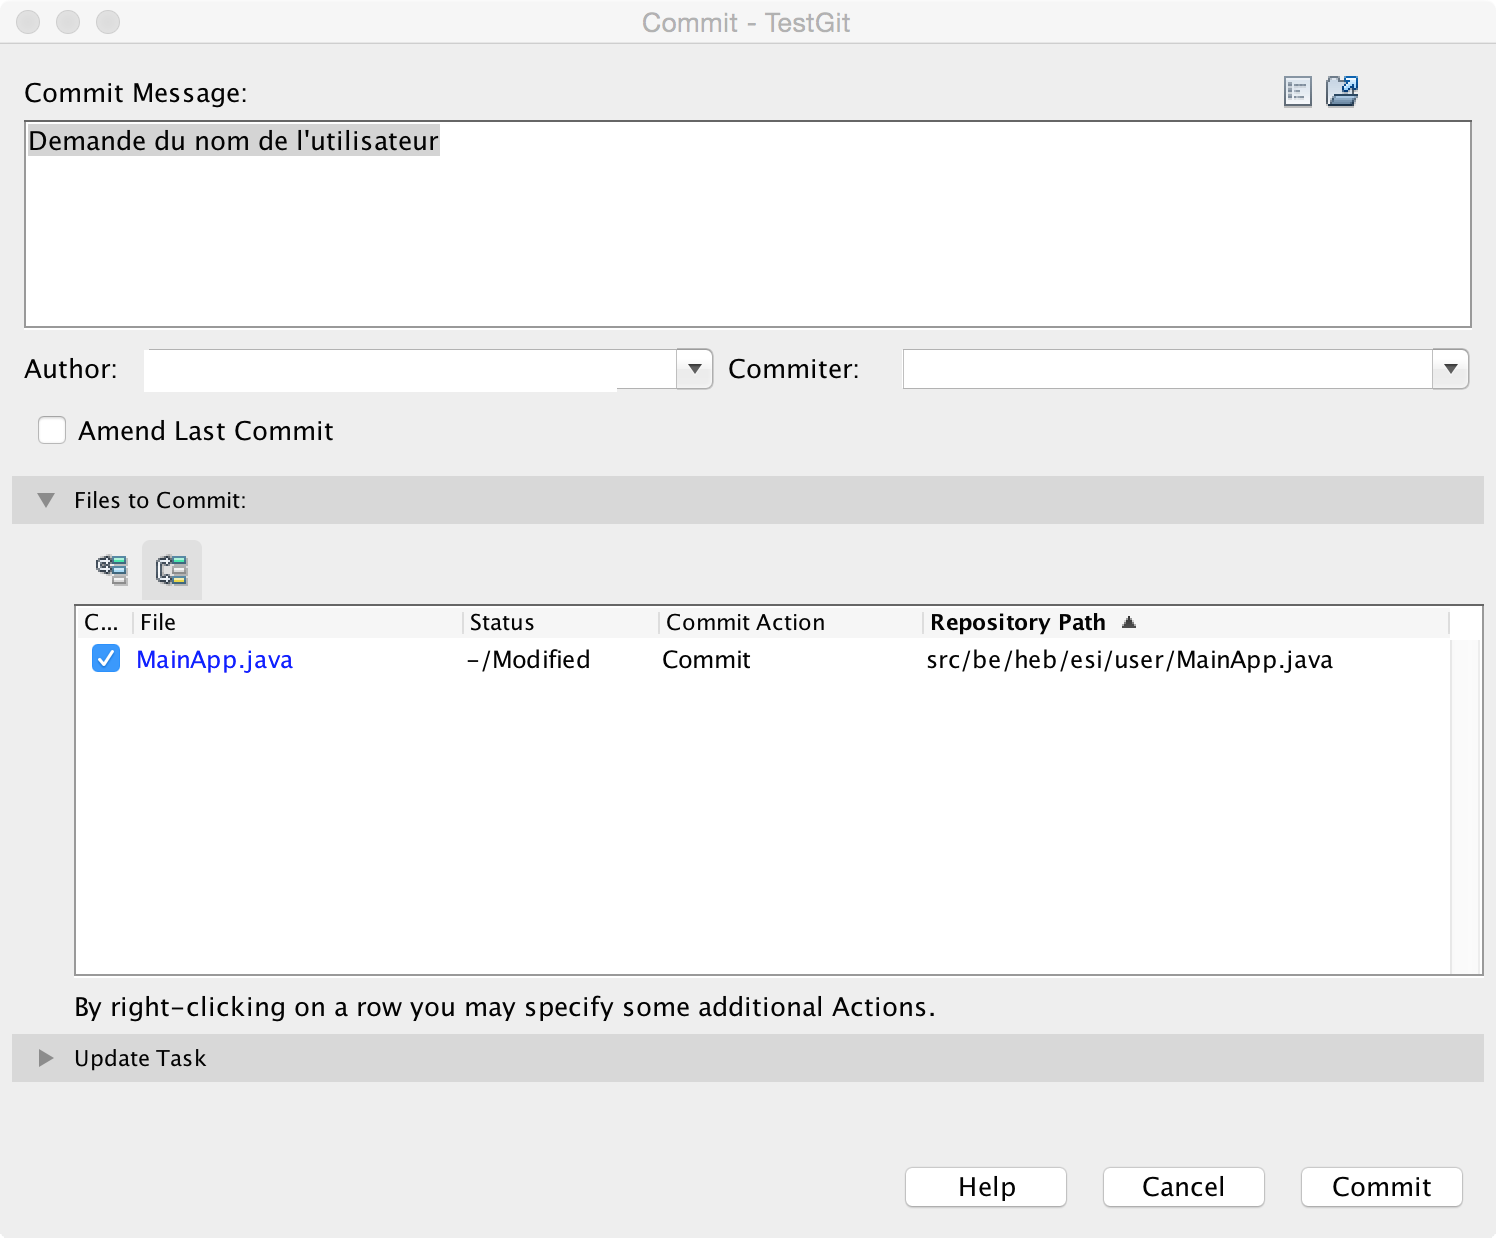
\includegraphics[width=.7\textwidth]{image/NetBeans_Project_031.png}
		\end{center}
	\end{steps}
	Comme vous le constatez sur l'écran de validation des commits, 
	un seul fichier a été modifié : \samp{MainApp.java}.
\end{Tutoriel}

%==========================
\section{Le serveur gitlab}
%==========================

Pour l'instant l'historique de votre projet 
est enregistré dans un dossier caché de votre projet (\samp{.git}).
Il est possible d'utiliser git sans serveur pour conserver un historique en local
mais l'utilisation d'un serveur permet de développer sur différentes machines.
C'est ce que nous allons voir dans cette section.

Un \textbf{serveur git} nous permet principalement :
\begin{itemize}
	\item de pouvoir accéder facilement à notre projet sur différentes machines ;
	\item de contribuer à plusieurs sur un même projet ;
	\item de montrer publiquement le projet à toute la communauté dès lors qu'il est public.
\end{itemize}

Nous avons installé à l'école le serveur \bsc{Gitlab for ÉSI}.
\begin{center}
	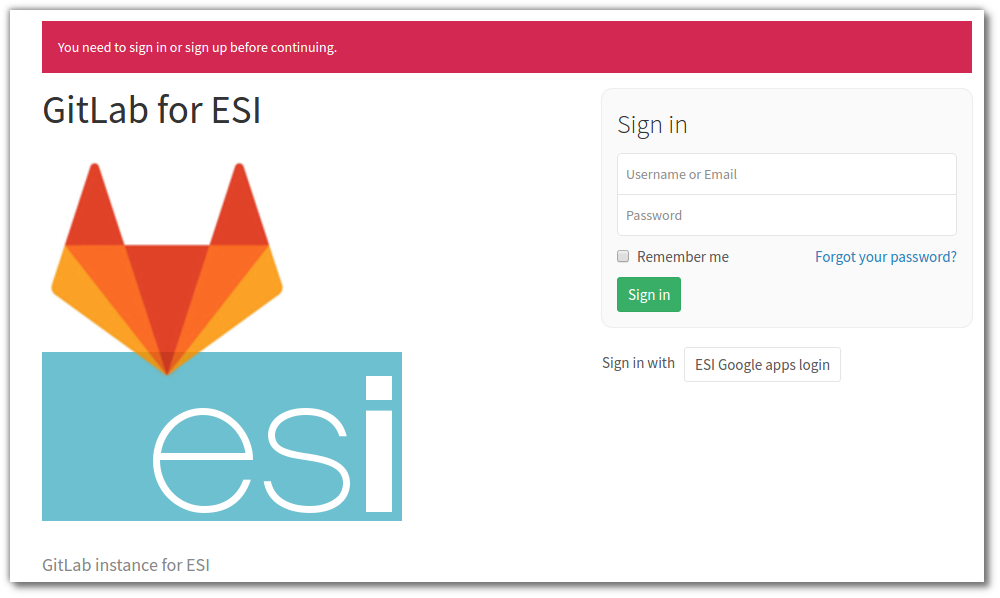
\includegraphics[width=.5\textwidth]{image/gitlab.png}
\end{center}

\begin{Tutoriel}{S'identifier sur le serveur}
%------------------------------------------------------------------
	Voyons comment s'identifier sur le serveur.
	\begin{steps}
	\item 
		Rendez-vous sur le serveur
		\url{https://git.esi-bru.be}
		et identifiez-vous en cliquant sur le bouton :
		\samp{ESI Google apps login}.
	\end{steps}
	Pour vous faciliter les opérations ultérieures,
	il est important de définir un mot de passe propre à ce serveur.
	Pour cela,
	\begin{steps}
	\item Cliquez sur le menu en haut à droite ;
	\item choisissez \samp{Profile settings}
			puis \samp{Password} ;
	\item Cliquez alors sur \samp{I forgot my password} et suivez la procédure.
	\end{steps}
\end{Tutoriel}

\begin{Tutoriel}{Création d'un dépôt sur le serveur}
%------------------------------------------------------------------
	Créons sur \bsc{gitlab} un \textbf{dépôt} 
	qui va pouvoir accueillir notre projet dans toutes ses versions.
	\begin{steps}
	\item 
		Sur la page d'accueil de votre compte GitLab, 
		vous trouverez un bouton dans le coin supérieur droit 
		vous permettant de créer des nouveaux projets.
		Cliquez dessus.
		\begin{center}
			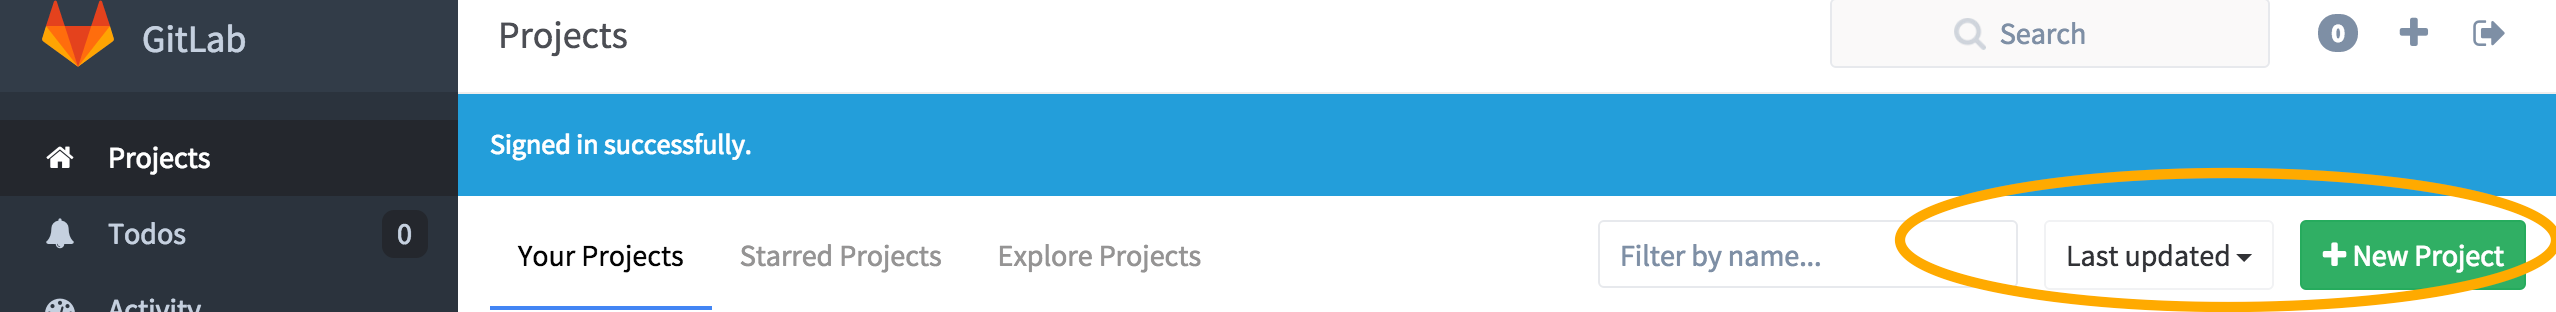
\includegraphics[width=.5\textwidth]{image/GitLabCreateProject00.png}
		\end{center}
	\item 
		Donnez à ce projet le nom : \samp{Dev1TdGit}
		et confirmez la création du projet.
		Vous êtes redirigé vers la page d'accueil du projet.
		\begin{center}
			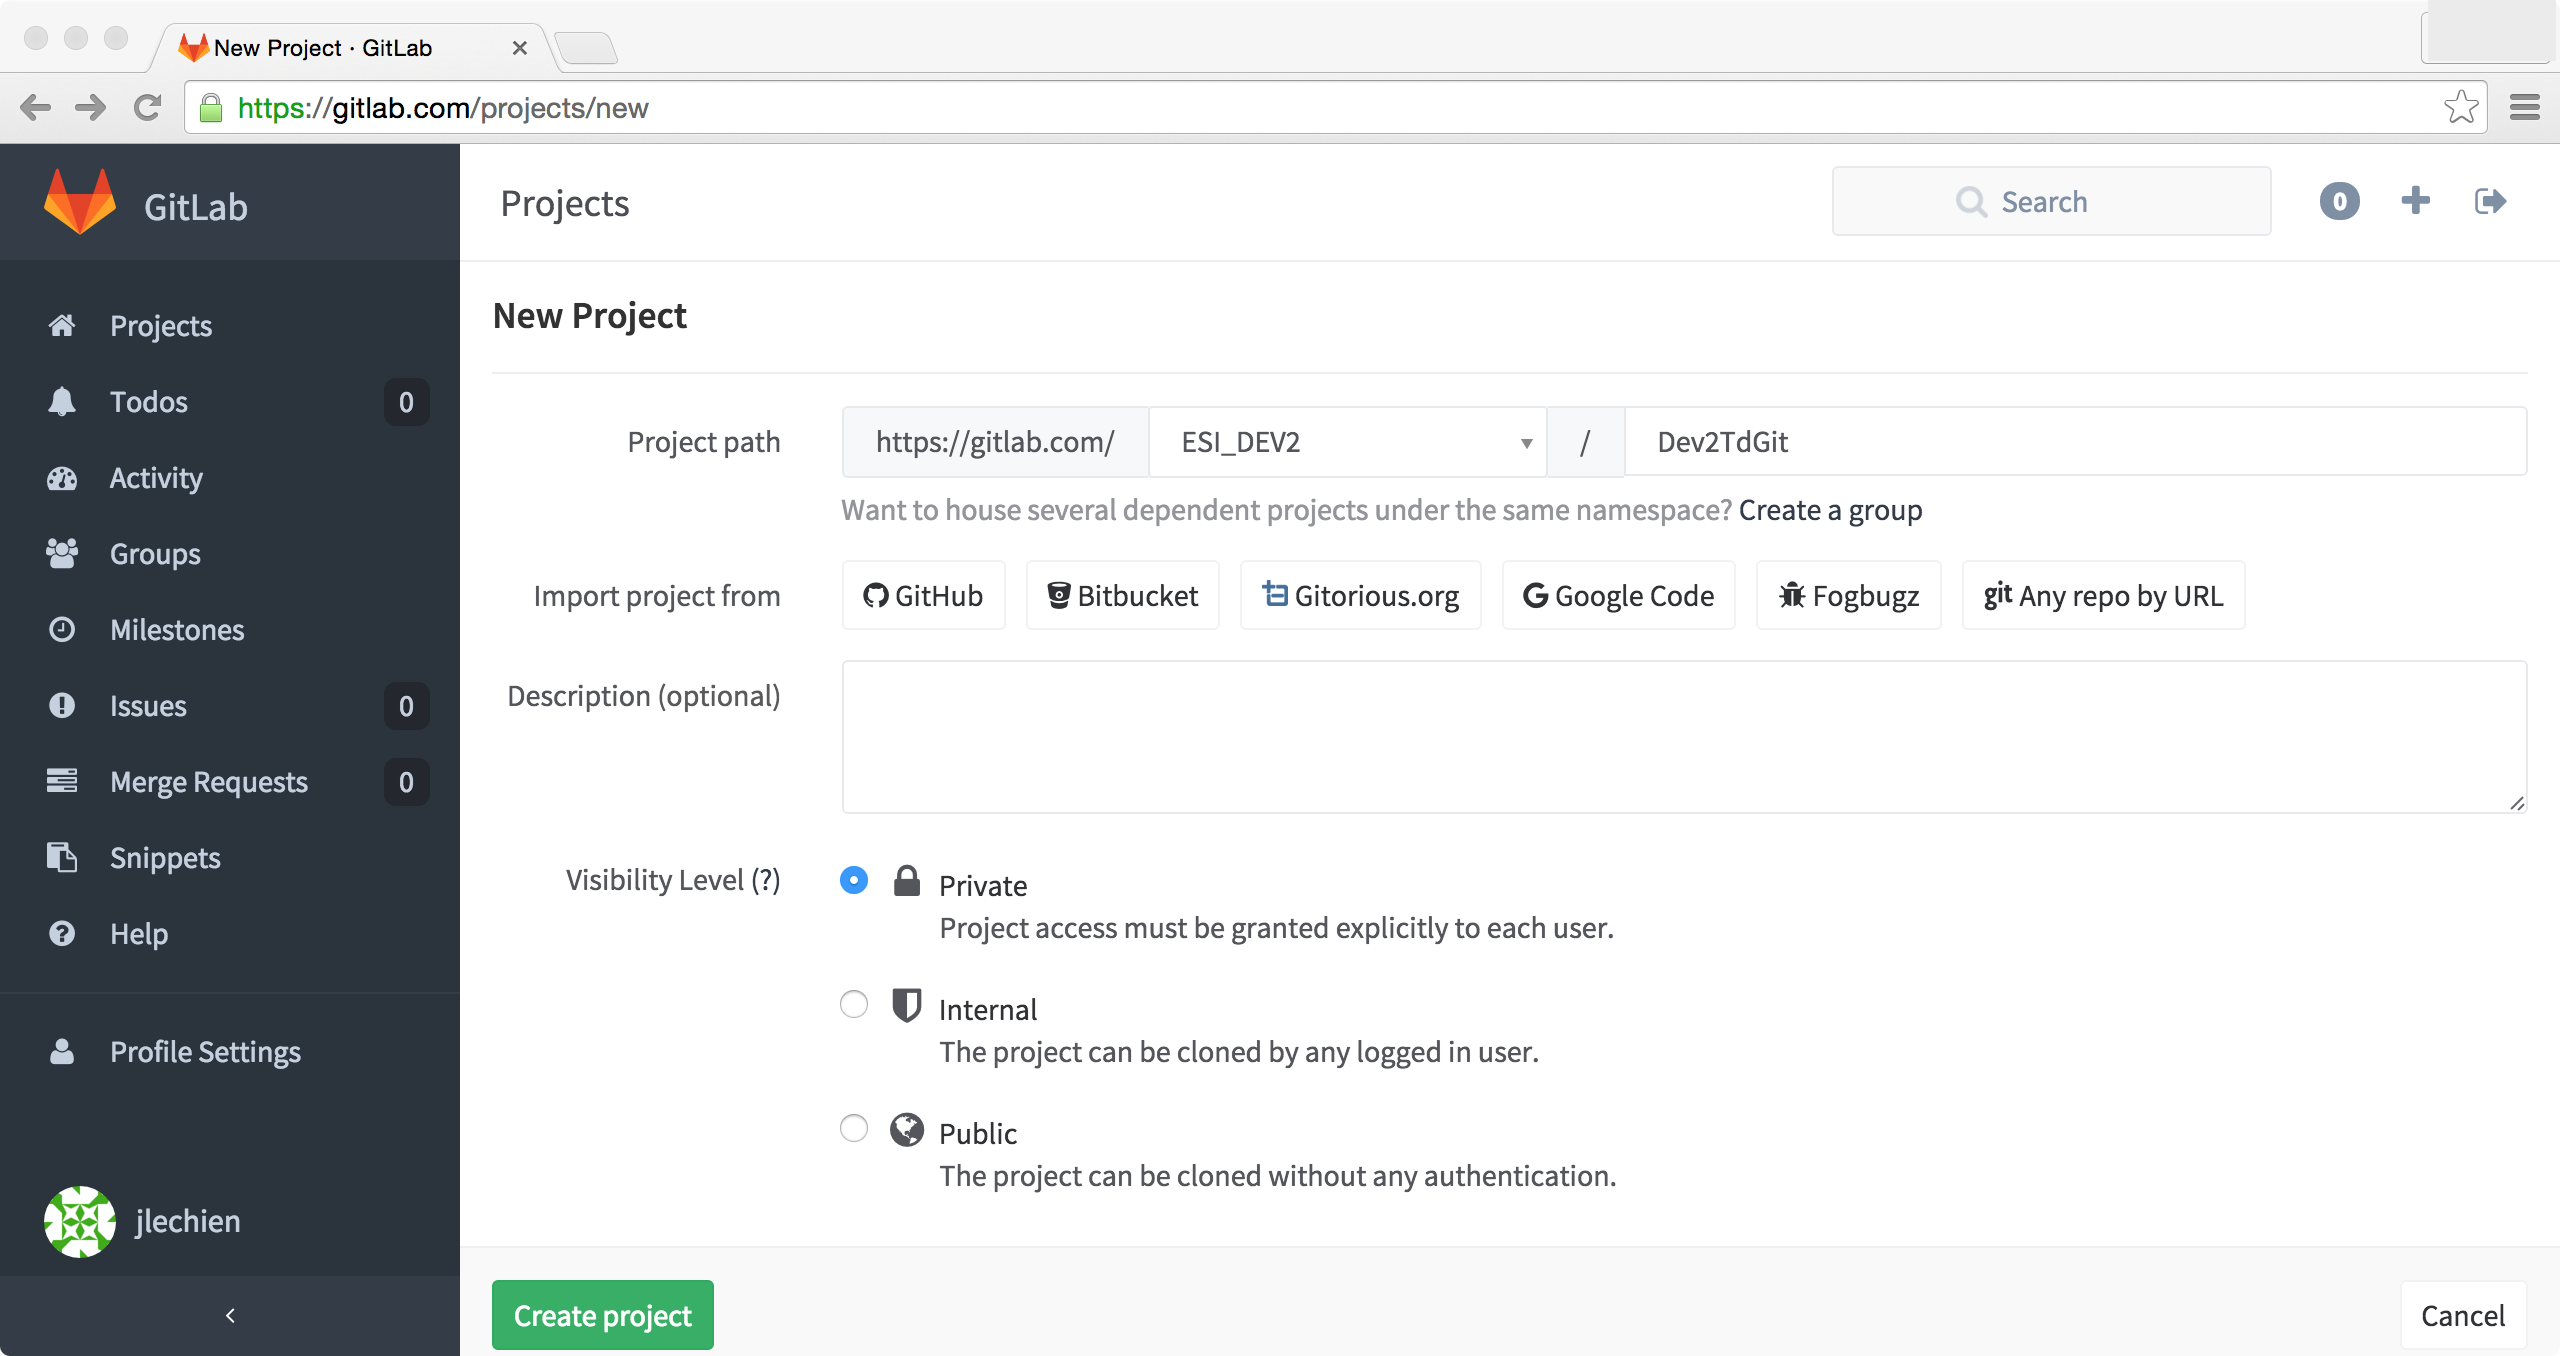
\includegraphics[width=.5\textwidth]{image/GitLabCreateProject01.png}
		\end{center}
	\end{steps}
\end{Tutoriel}

\begin{Tutoriel}{Premier push}
%------------------------------------------------------------------
	Il est temps de sauver l'historique de votre projet \bsc{Netbeans} 
	sur le serveur \bsc{GitLab}.

	\begin{infoit}{Push}
		Un \textbf{push} 
		consiste à envoyer sur le serveur 
		tous les nouveaux commits effectués localement.
	\end{infoit}

	Pour effectuer ce push :
	\begin{steps}
	\item 
		Sur la page d'accueil de votre dépôt GitLab,
		récupérez l'url \samp{https} de ce dépôt.
 		Elle sera du type
		\url{https://git.esi-bru.be/g12345/Dev1TdGit.git}.
		Le plus simple est de la copier dans le presse-papier.
	\item 
		Dans NetBeans :
		\begin{steps}
		\item Dans l'onglet \samp{Projects} cliquez droit sur le projet.
		\item Choisissez l'option \samp{Git}, 
			suivi de \samp{Remote} et enfin \samp{Push...}
		\end{steps}
	\end{steps}
	Comme c'est le tout premier \emph{push} pour ce projet,
	il va falloir indiquer à \bsc{Netbeans} quel dépôt utilisé.
	Les \emph{push} suivants seront plus immédiats.
	\begin{steps}
	\item 
		Dans \samp{Remote Repository} : 
		\begin{steps}
			\item Copiez l'url \emph{https} de votre projet
				(celui que vous venez de copier) ;
			\item Entrez votre \samp{username}
			\item Ainsi que votre \samp{password} (défini un peu plus tôt).
			\item Cliquez sur \samp{Next>}
			\begin{center}
				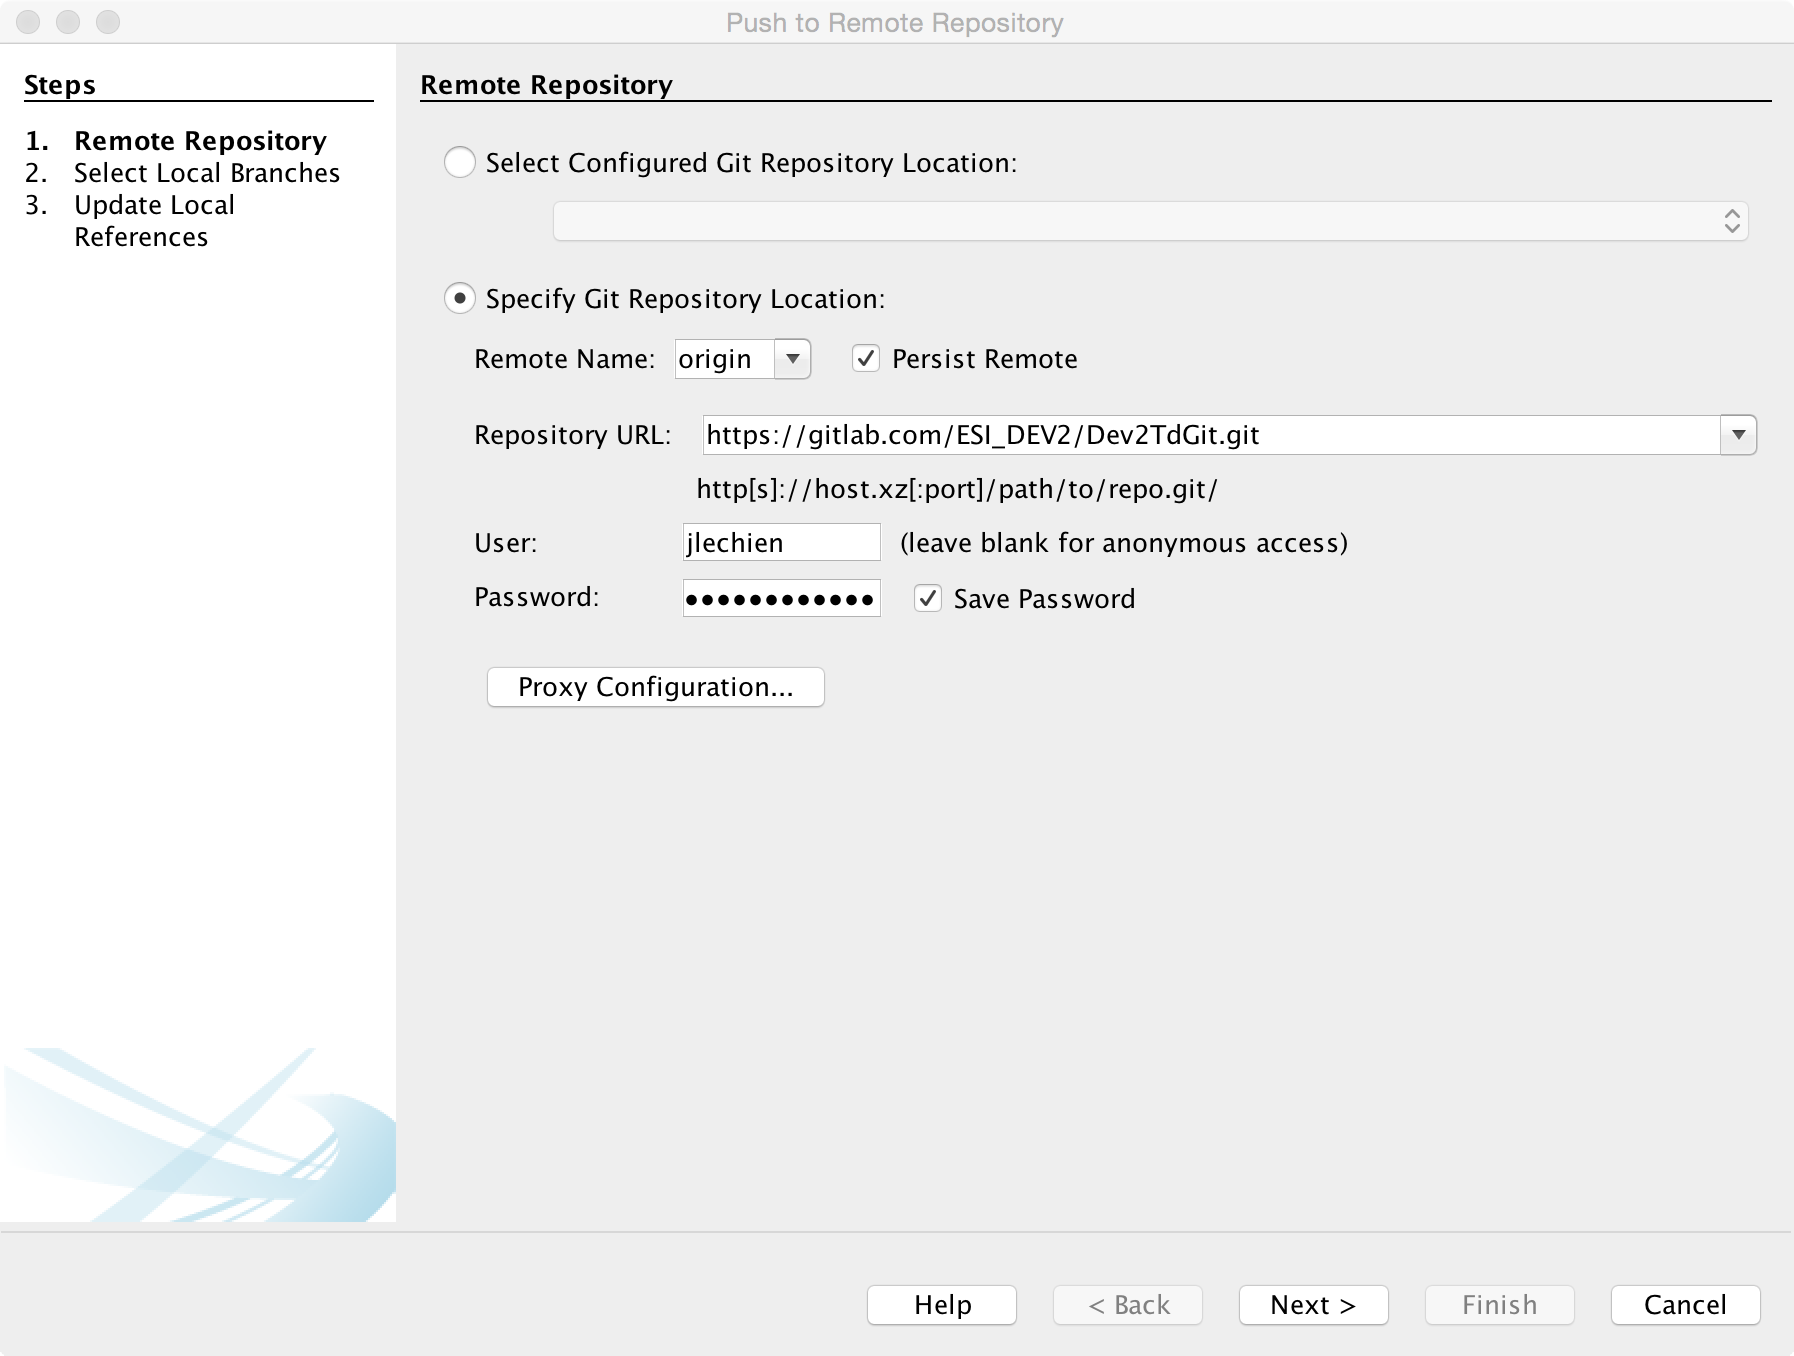
\includegraphics[width=.5\textwidth]{image/NetBeans_Push05.png}
			\end{center}		
		\end{steps}
	\item 
		Dans \samp{Local Branches} : 
		\begin{steps}
			\item Sélectionnez \samp{master -> master}
			\item Cliquez sur \samp{Next>}
			\begin{center}
				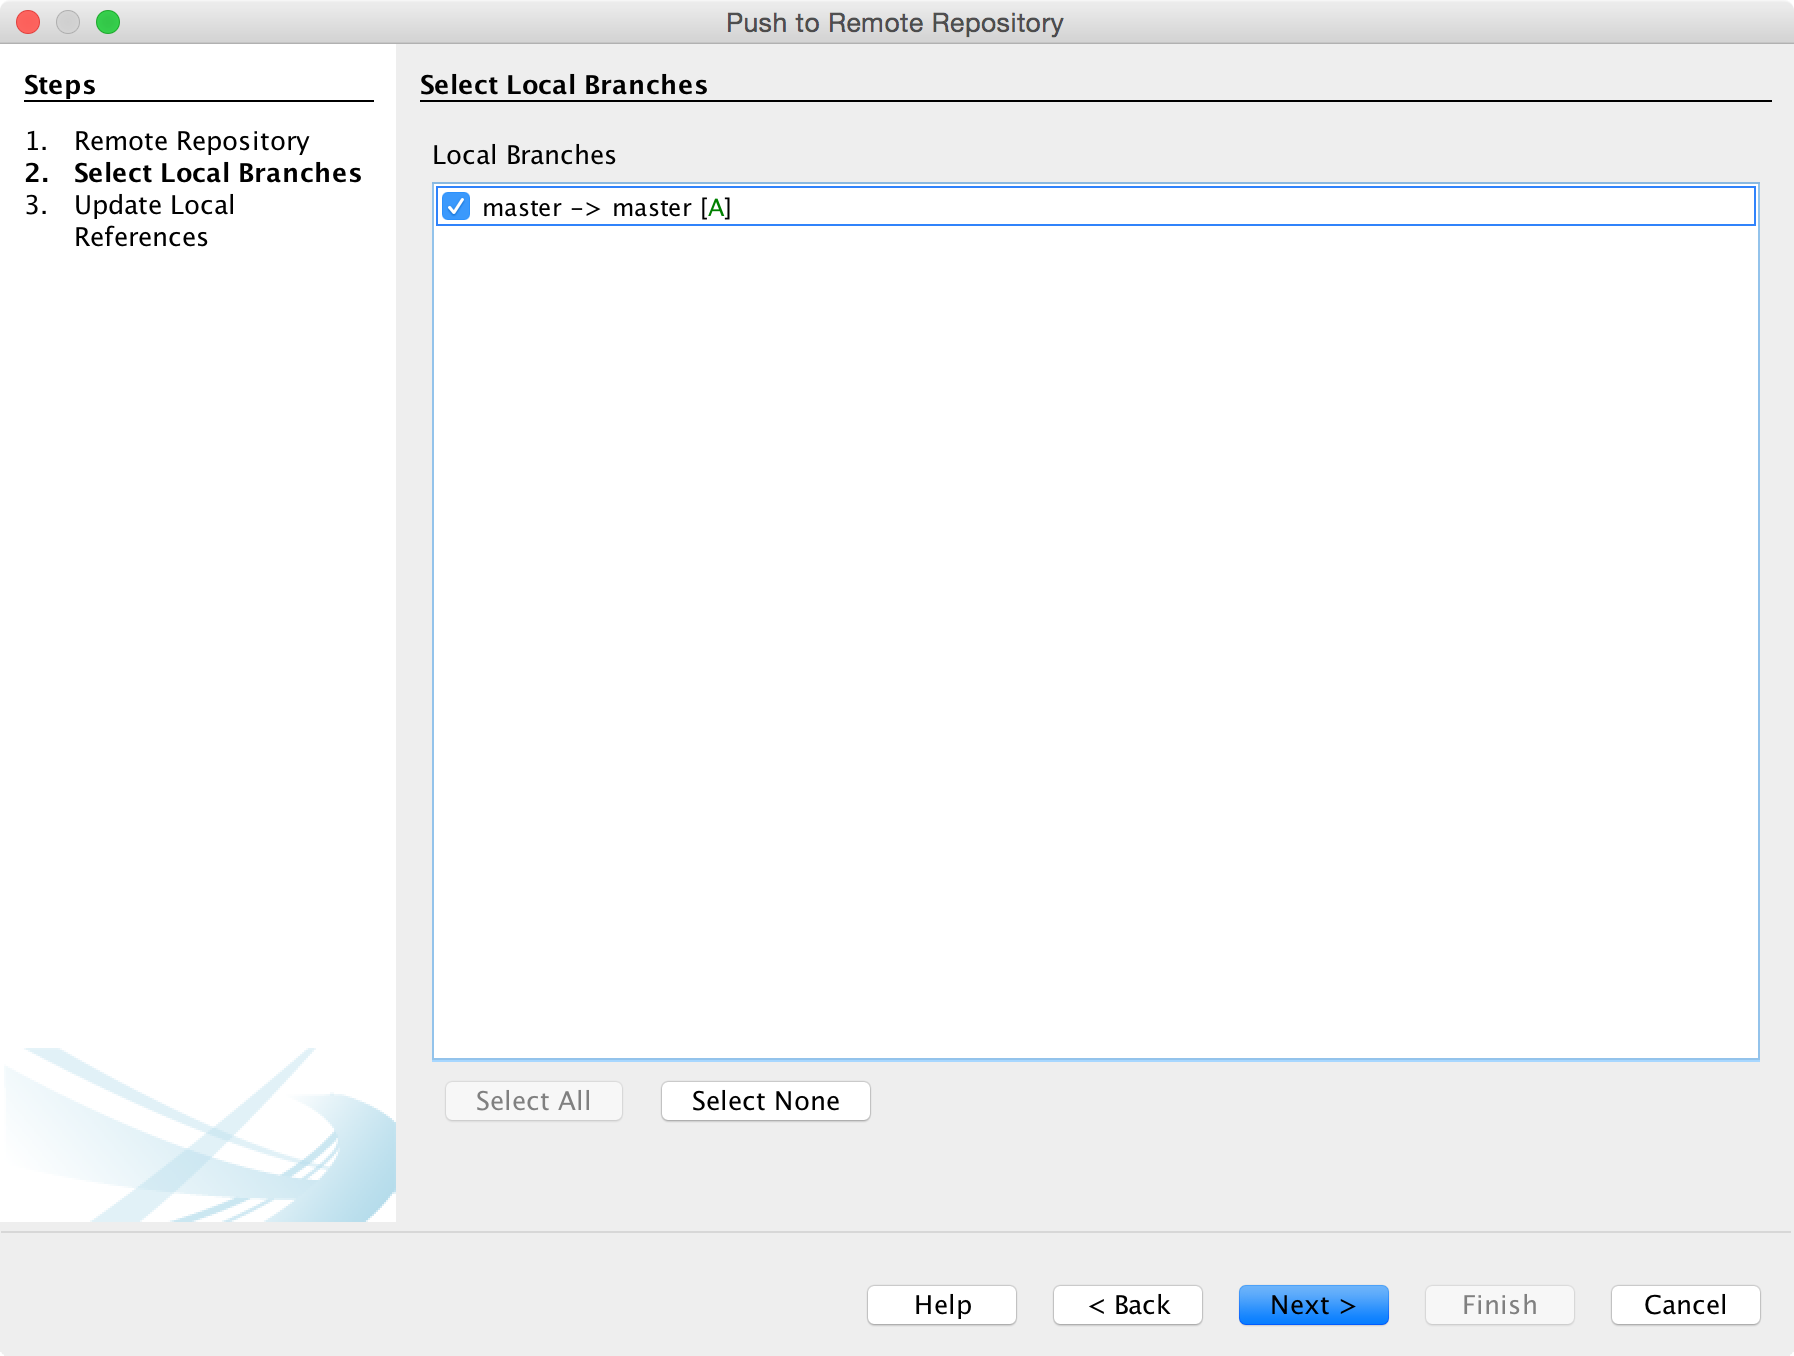
\includegraphics[width=.5\textwidth]{image/NetBeans_Push06.png}
			\end{center}		
		\end{steps}
	\item 
		Dans \samp{Update Local References} : 
		Il vous suffit de cliquer sur \samp{Finish}

		La première fois que vous effectuez un push, un popup apparait.
		Confirmez sans crainte.
		\begin{center}
			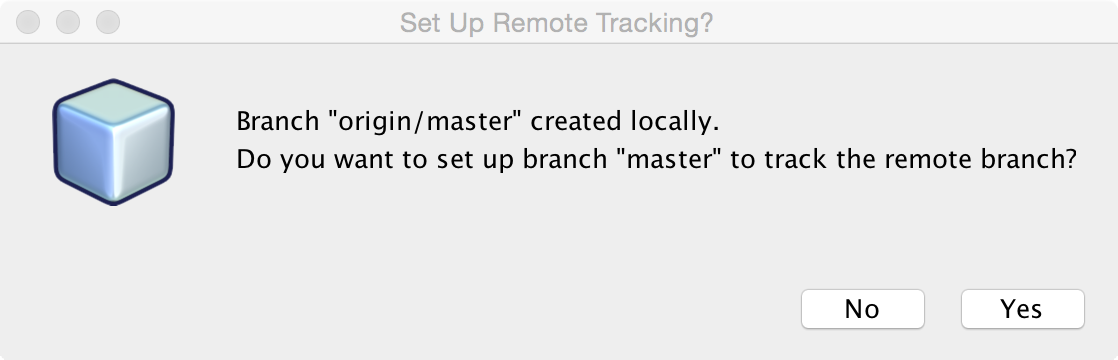
\includegraphics[width=.5\textwidth]{image/NetBeans_Push08.png}
		\end{center}
	\end{steps}
\end{Tutoriel}

\begin{alertit}{On ne push que ce qui est commité}
	Attention,
	lors du \emph{push}, 
	seuls les commits sont envoyés sur le serveur.
	Si vous avez sauver un fichier 
	mais que vous ne l'avez pas inclus dans un commit,
	il ne sera pas envoyé sur le serveur !
\end{alertit}

\begin{Tutoriel}{Changement sur le serveur}
	L'effet du \emph{push} peut être constaté sur le serveur.
	\begin{steps}
	\item
		Visitez la page principale de votre projet sur le serveur gitlab.
		Le résultat de votre \samp{push} apparait sur la page d'accueil.
		\begin{center}
			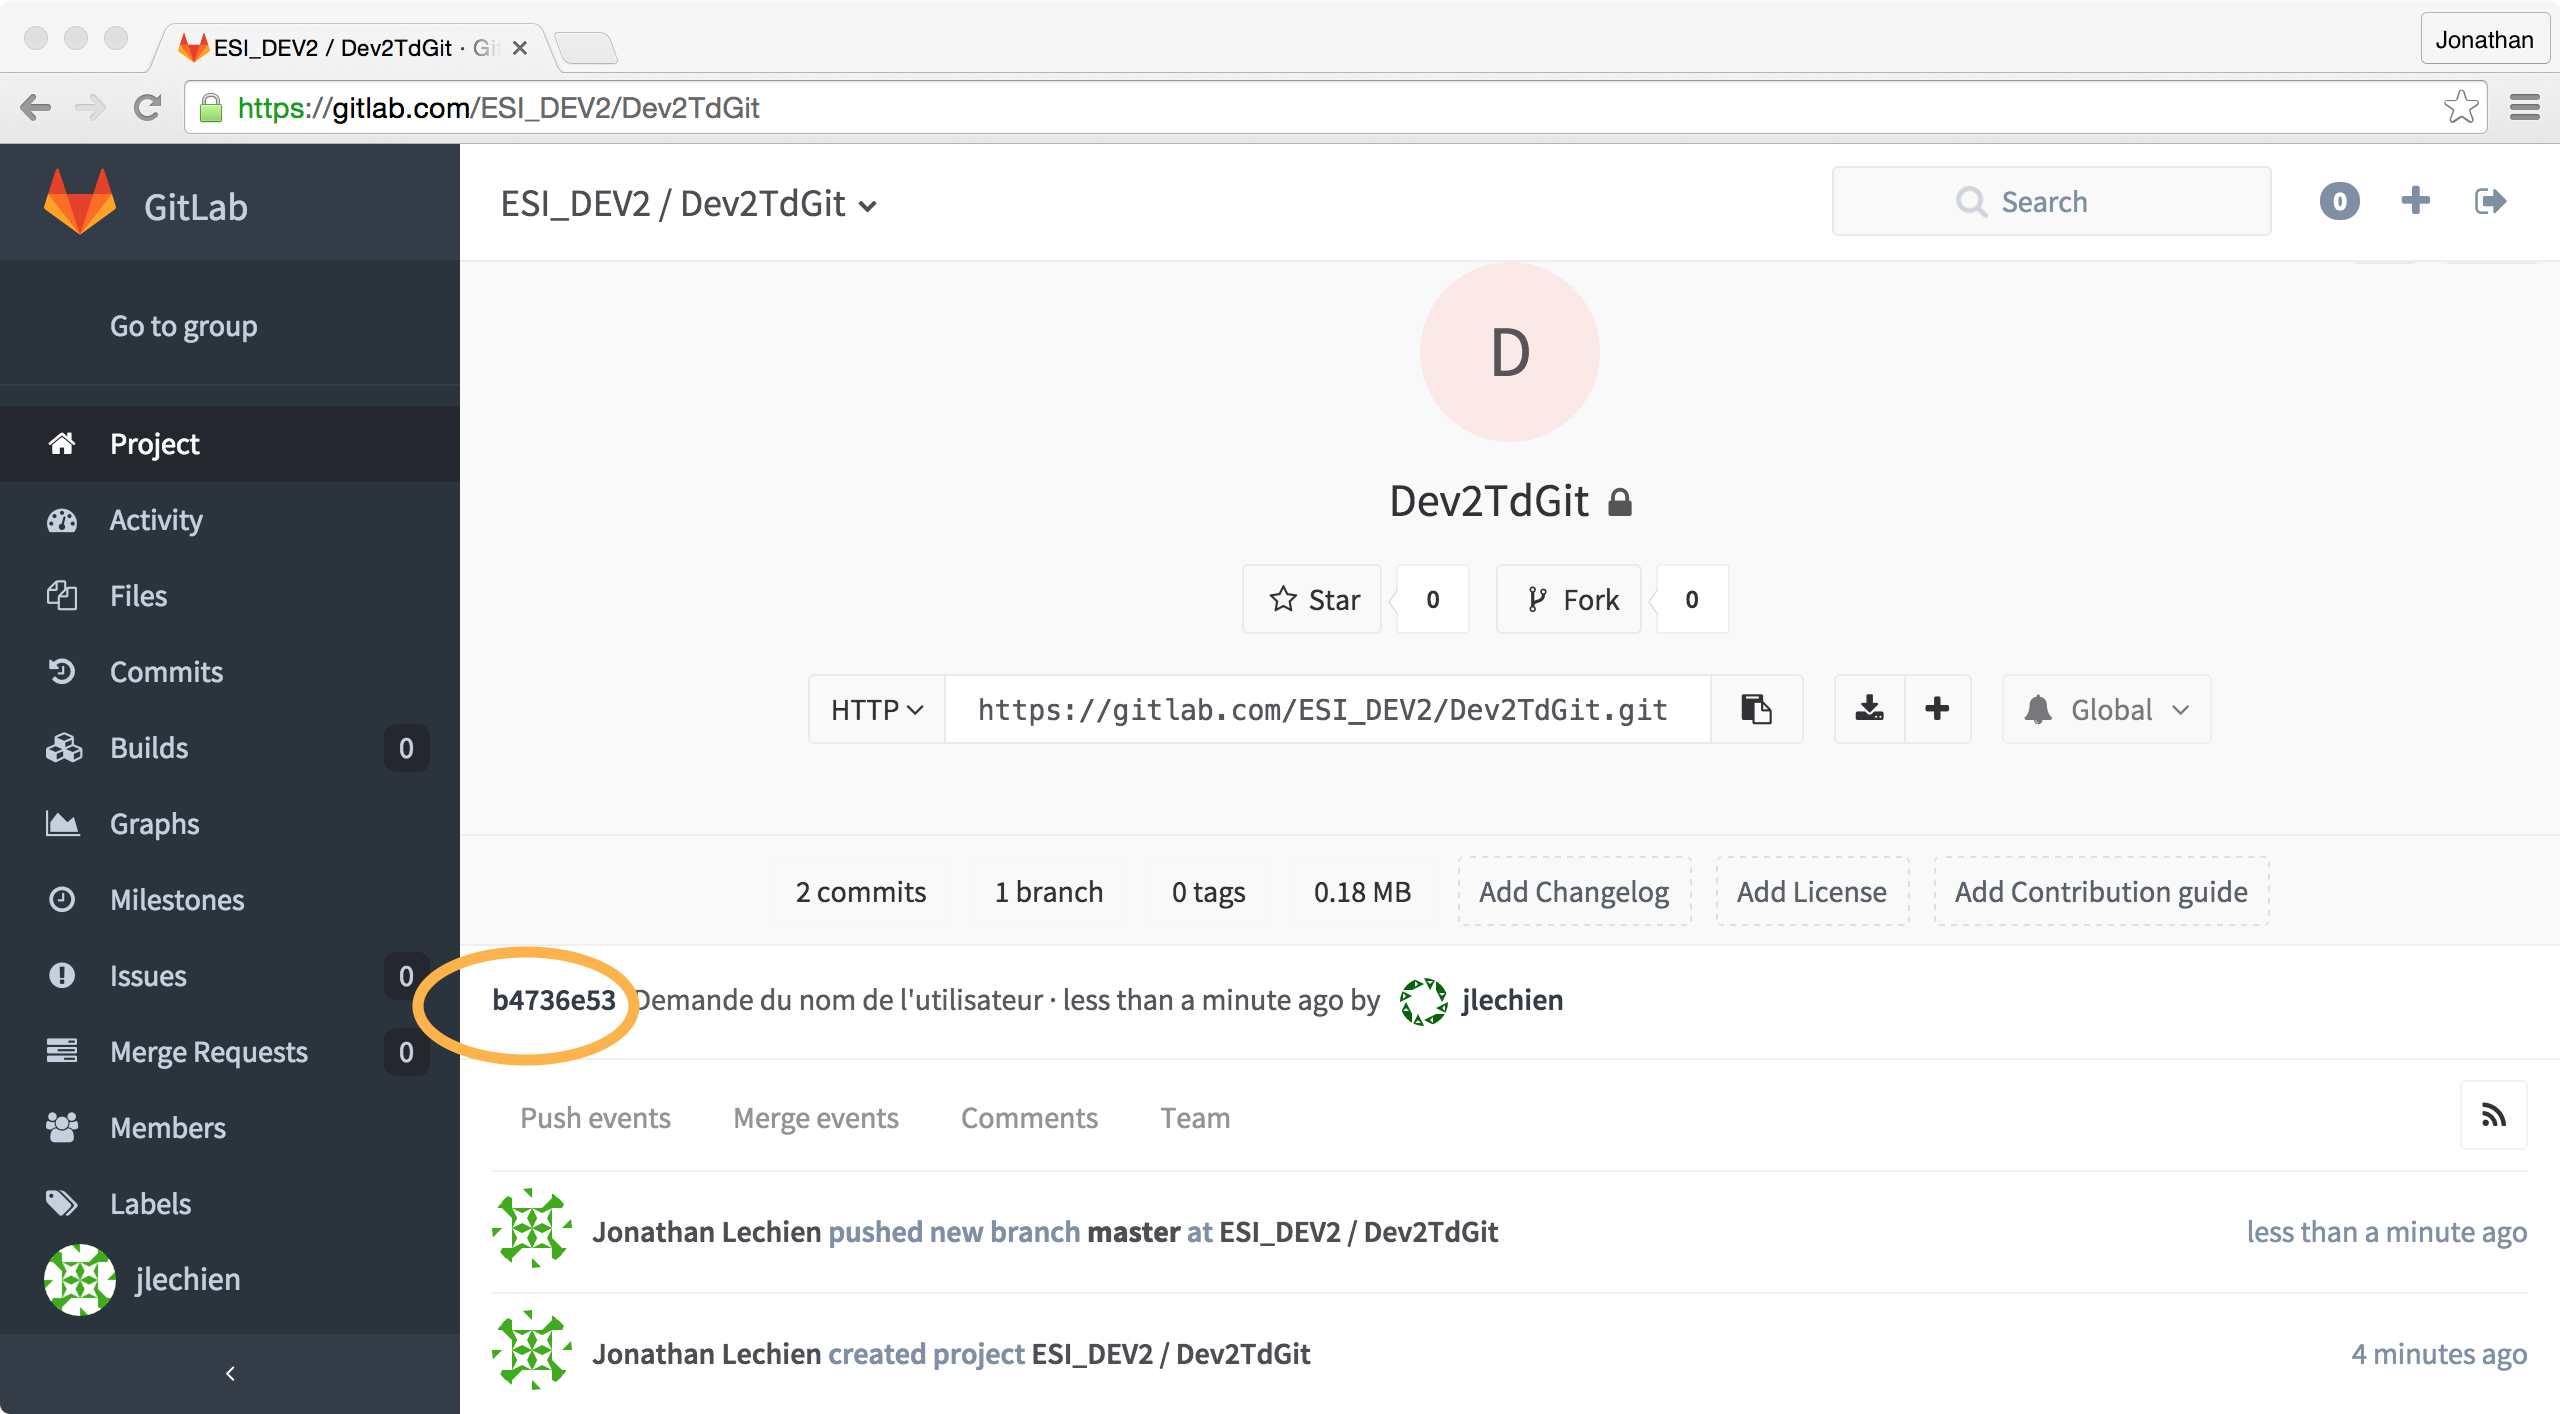
\includegraphics[width=.7\textwidth]{image/NetBeans_Push09.png}
		\end{center}
	\item 
		Via le menu \samp{Files}, 
		vous pouvez visualiser les fichiers déposés sur le serveur
		et leur contenu.
		\begin{center}
			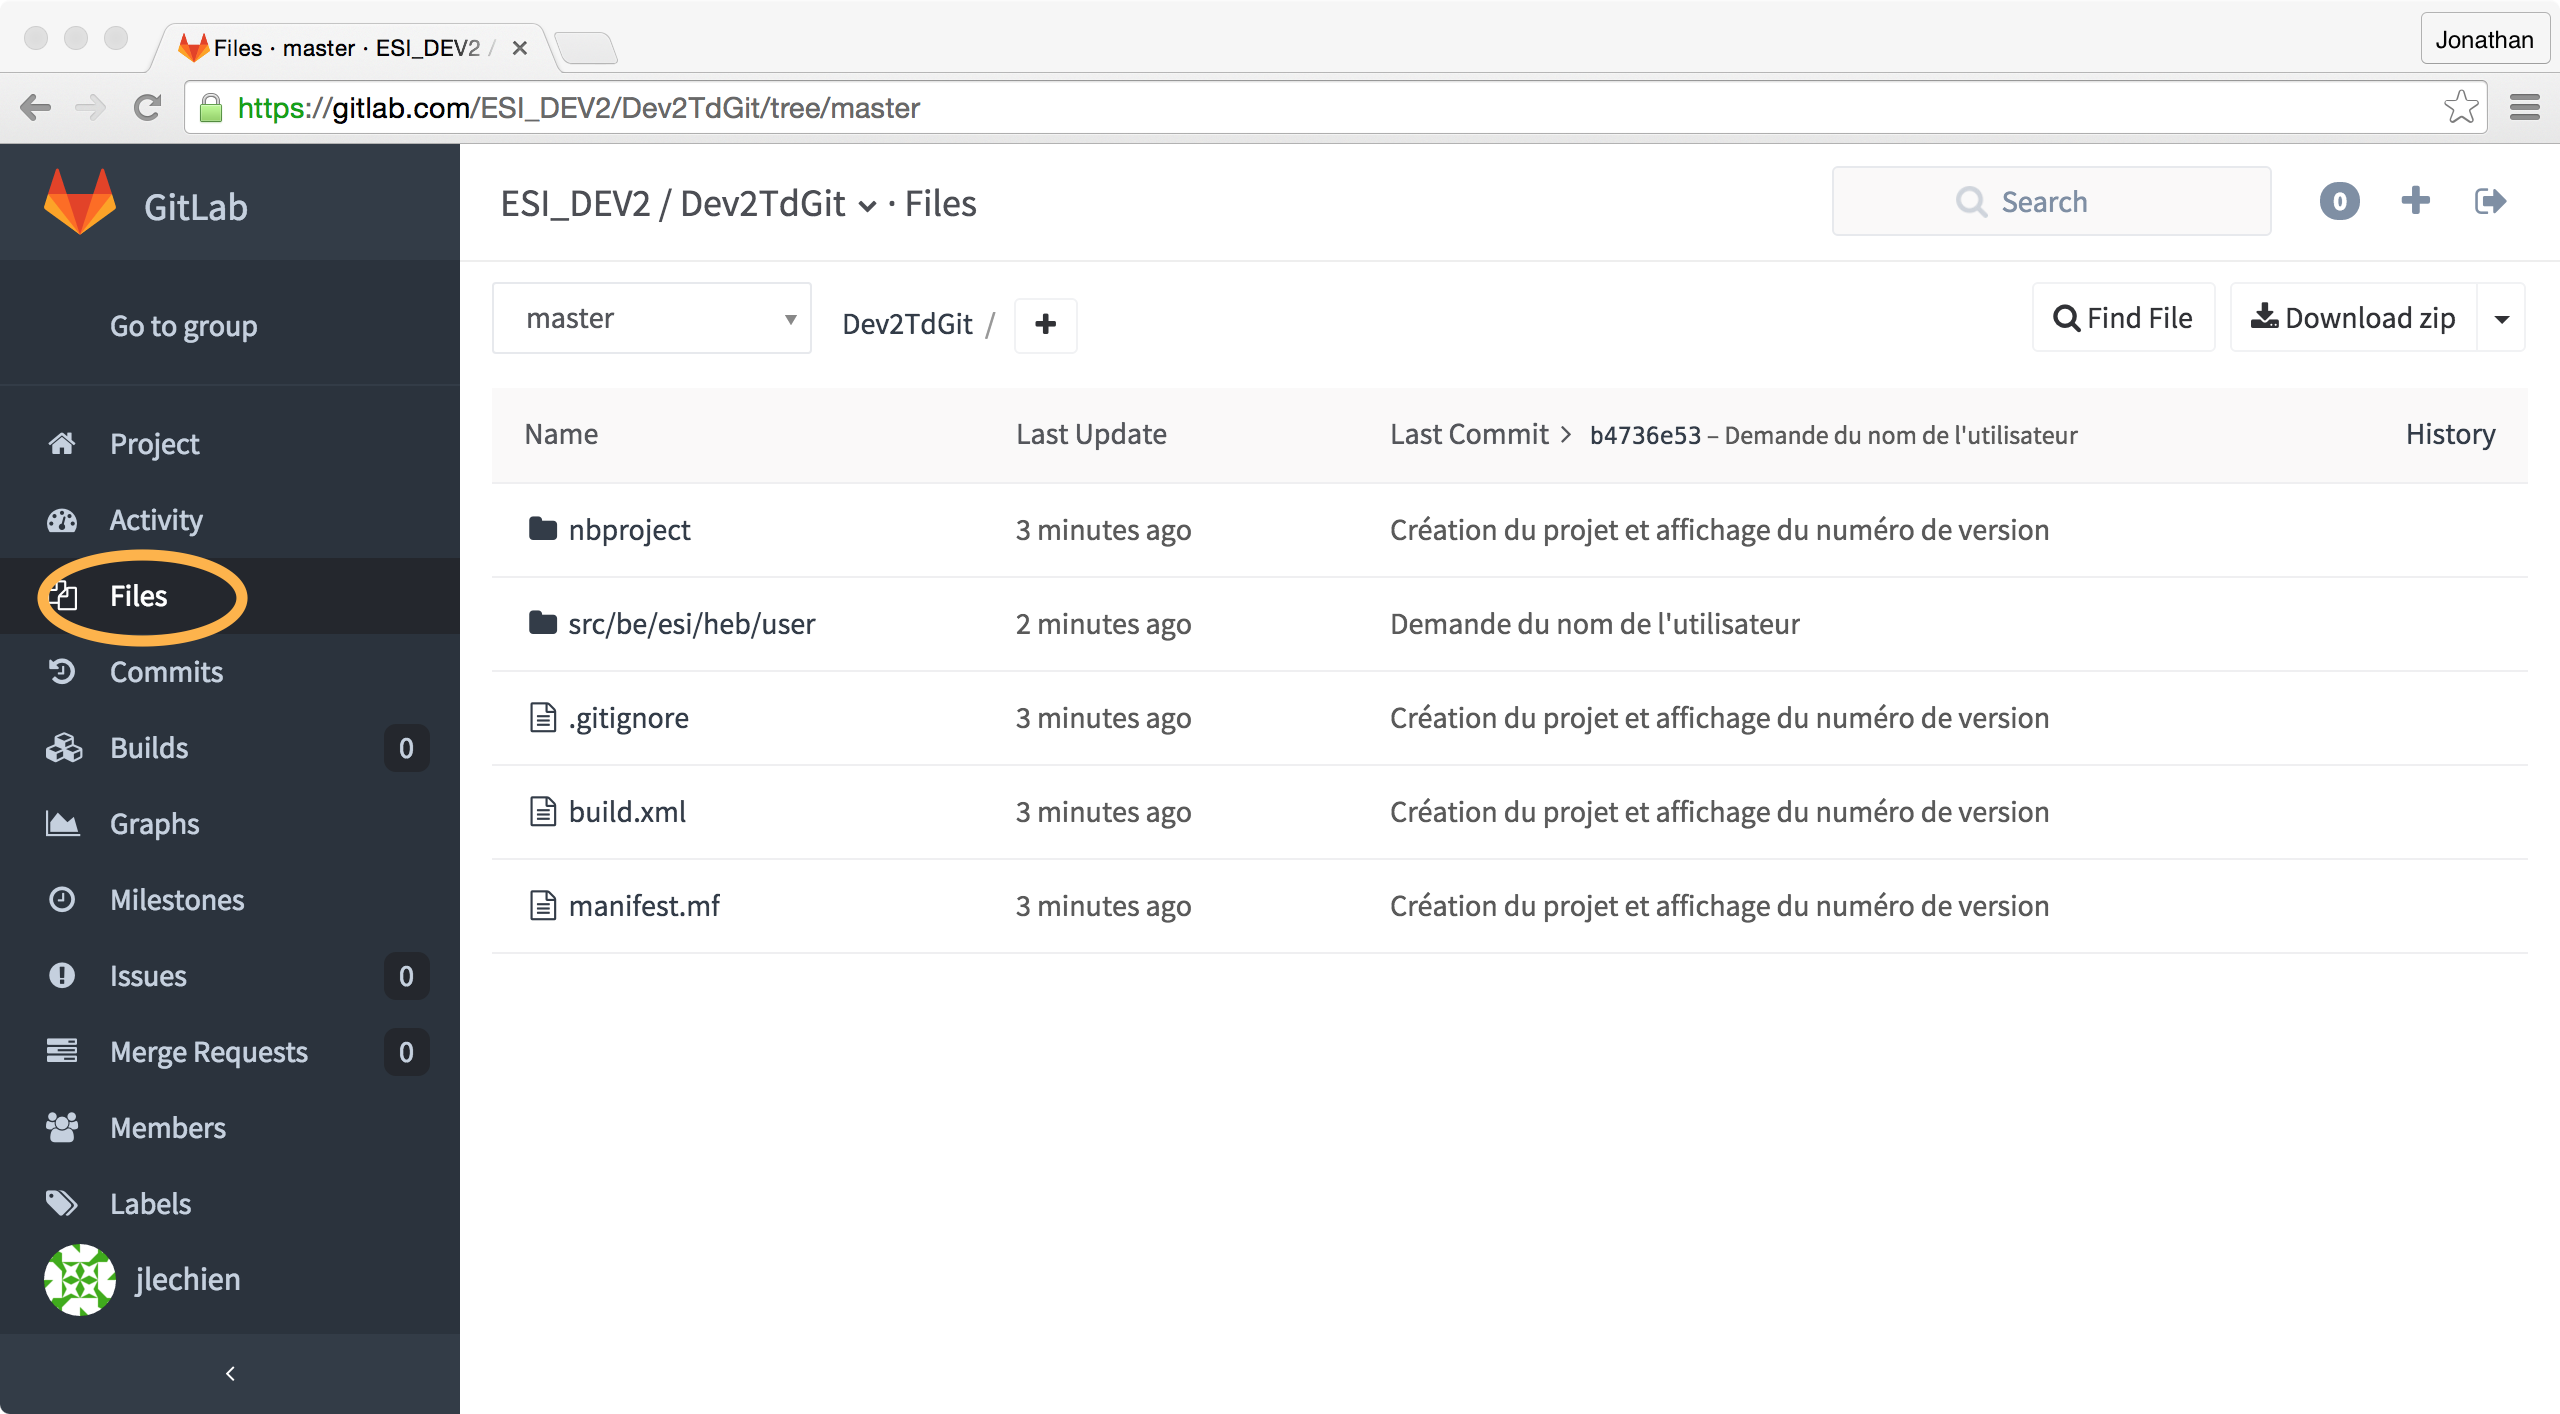
\includegraphics[width=.7\textwidth]{image/NetBeans_Push10.png}
		\end{center}
	\end{steps}
\end{Tutoriel}

\newpage
%==============================
\section{Changement de machine}
%==============================

Que se passe-t'il si on se connecte sur une machine 
où ne se trouve pas encore le projet ?
Comment le récupérer pour pouvoir continuer à travailler ?
C'est ce que nous allons expérimenter dans cette section.

Pour ce faire, vous devez donc vous déconnecter de cette machine
pour vous connecter sur une autre et reprendre le TD à cet endroit.

À tout de suite\dots{}

\begin{Tutoriel}{Cloner un projet}
	Vous voici sur une nouvelle machine et vous aimeriez récupérer
	ce qui a été déposé sur le serveur \bsc{gitlab}.

	\begin{infoit}{Clone}
		Un \textbf{clone}
		consiste à récupérer de \bsc{gitlab}%
		\footnote{ou tout autre serveur du même genre.}
		le contenu \textbf{complet} d'un dépôt (tous les commits).
		On l'utilise lorsqu'il n'y a encore \textbf{rien} sur la machine.
	\end{infoit}

	\begin{steps}
	\item 
		Dans NetBeans,
		choisissez \samp{Team/Git/Clone...}
		\begin{center}
			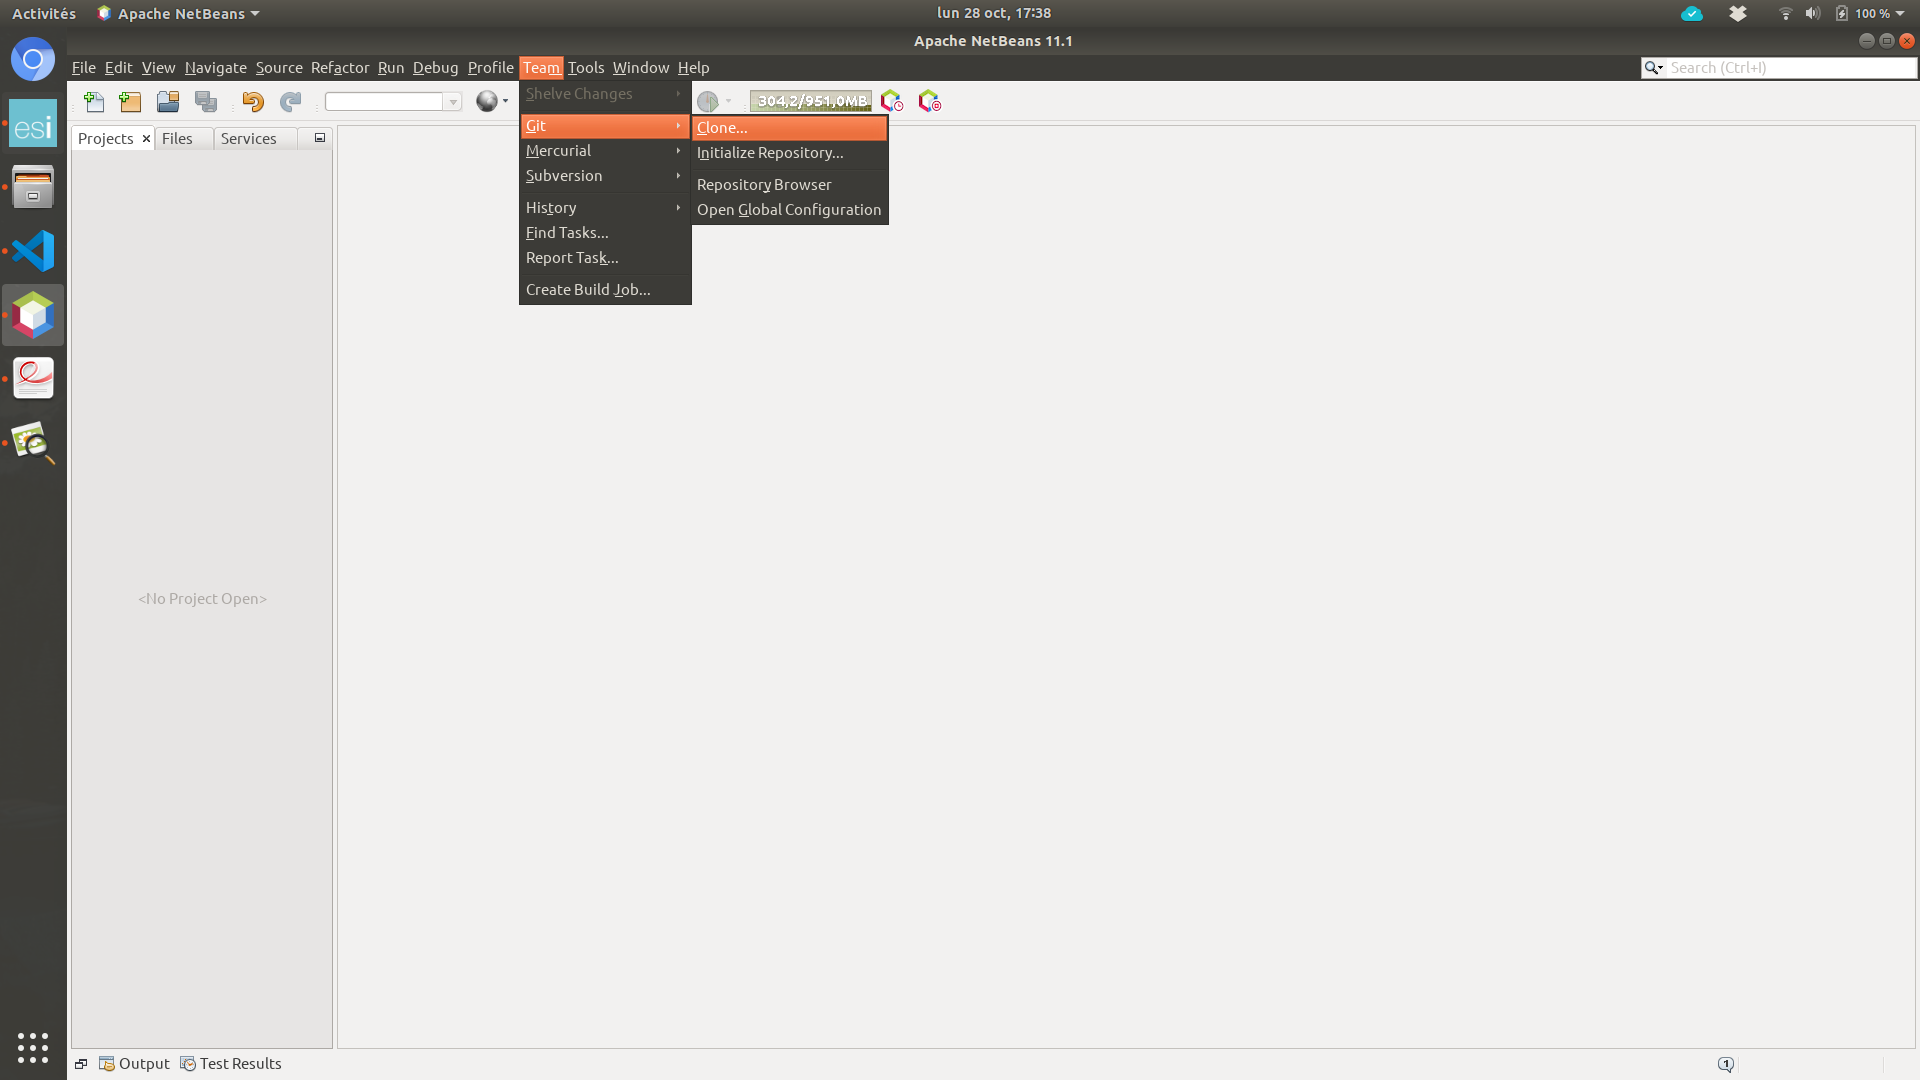
\includegraphics[width=.5\textwidth]{image/NetBeans_clone01.png}
		\end{center}
	\item 
		Vous êtes renvoyé vers l'écran de clonage.
		Pour terminer l'opération il suffit :
		\begin{steps}
		\item
			Dans \samp{Remote Repository} : 
			d'entrer l'url du dépôt, votre login et mot de passe
			et de choisir un répertoire pour l'enregistrer ;
			\begin{center}
				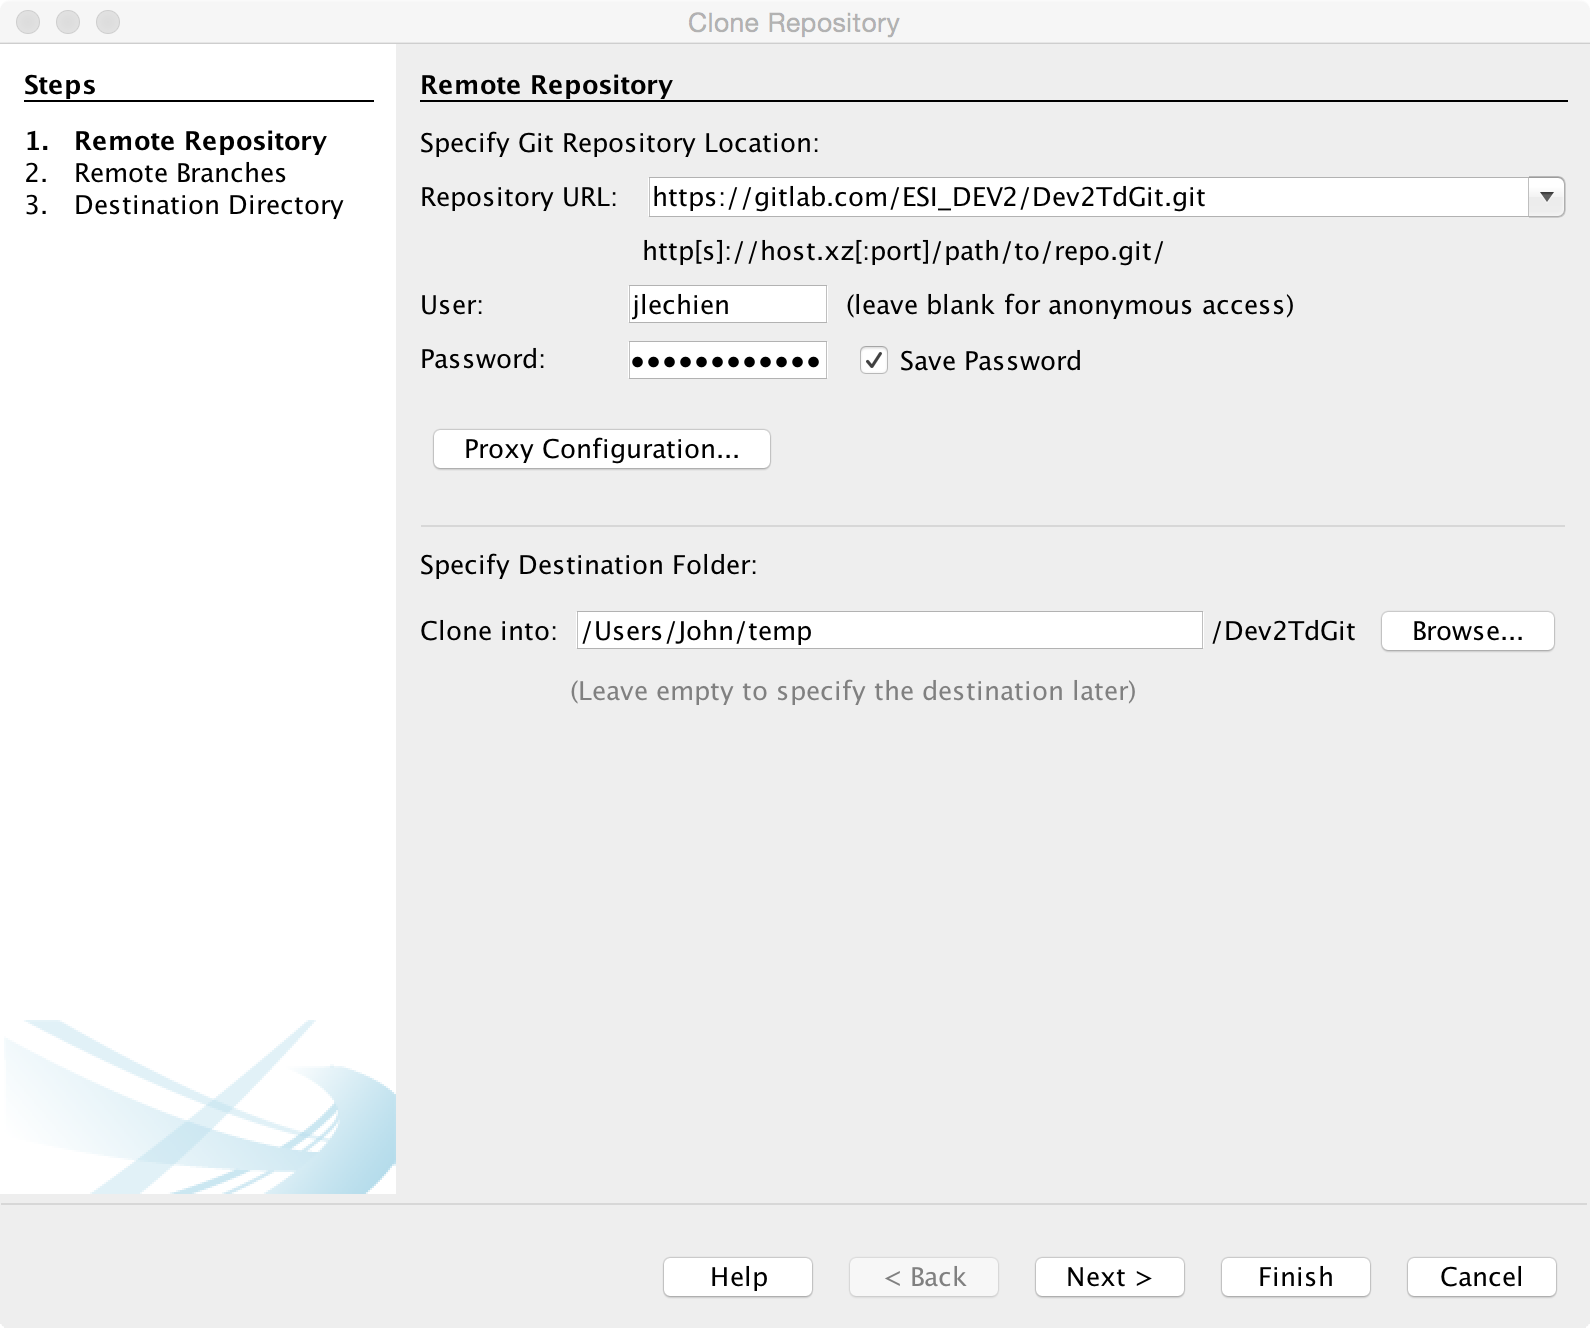
\includegraphics[width=.7\textwidth]{image/NetBeans_clone03.png}
			\end{center}
		\item
			Dans \samp{Remote Branches} : 
			de sélectionner l'option \samp{master} ;
			% \begin{center}
			% 	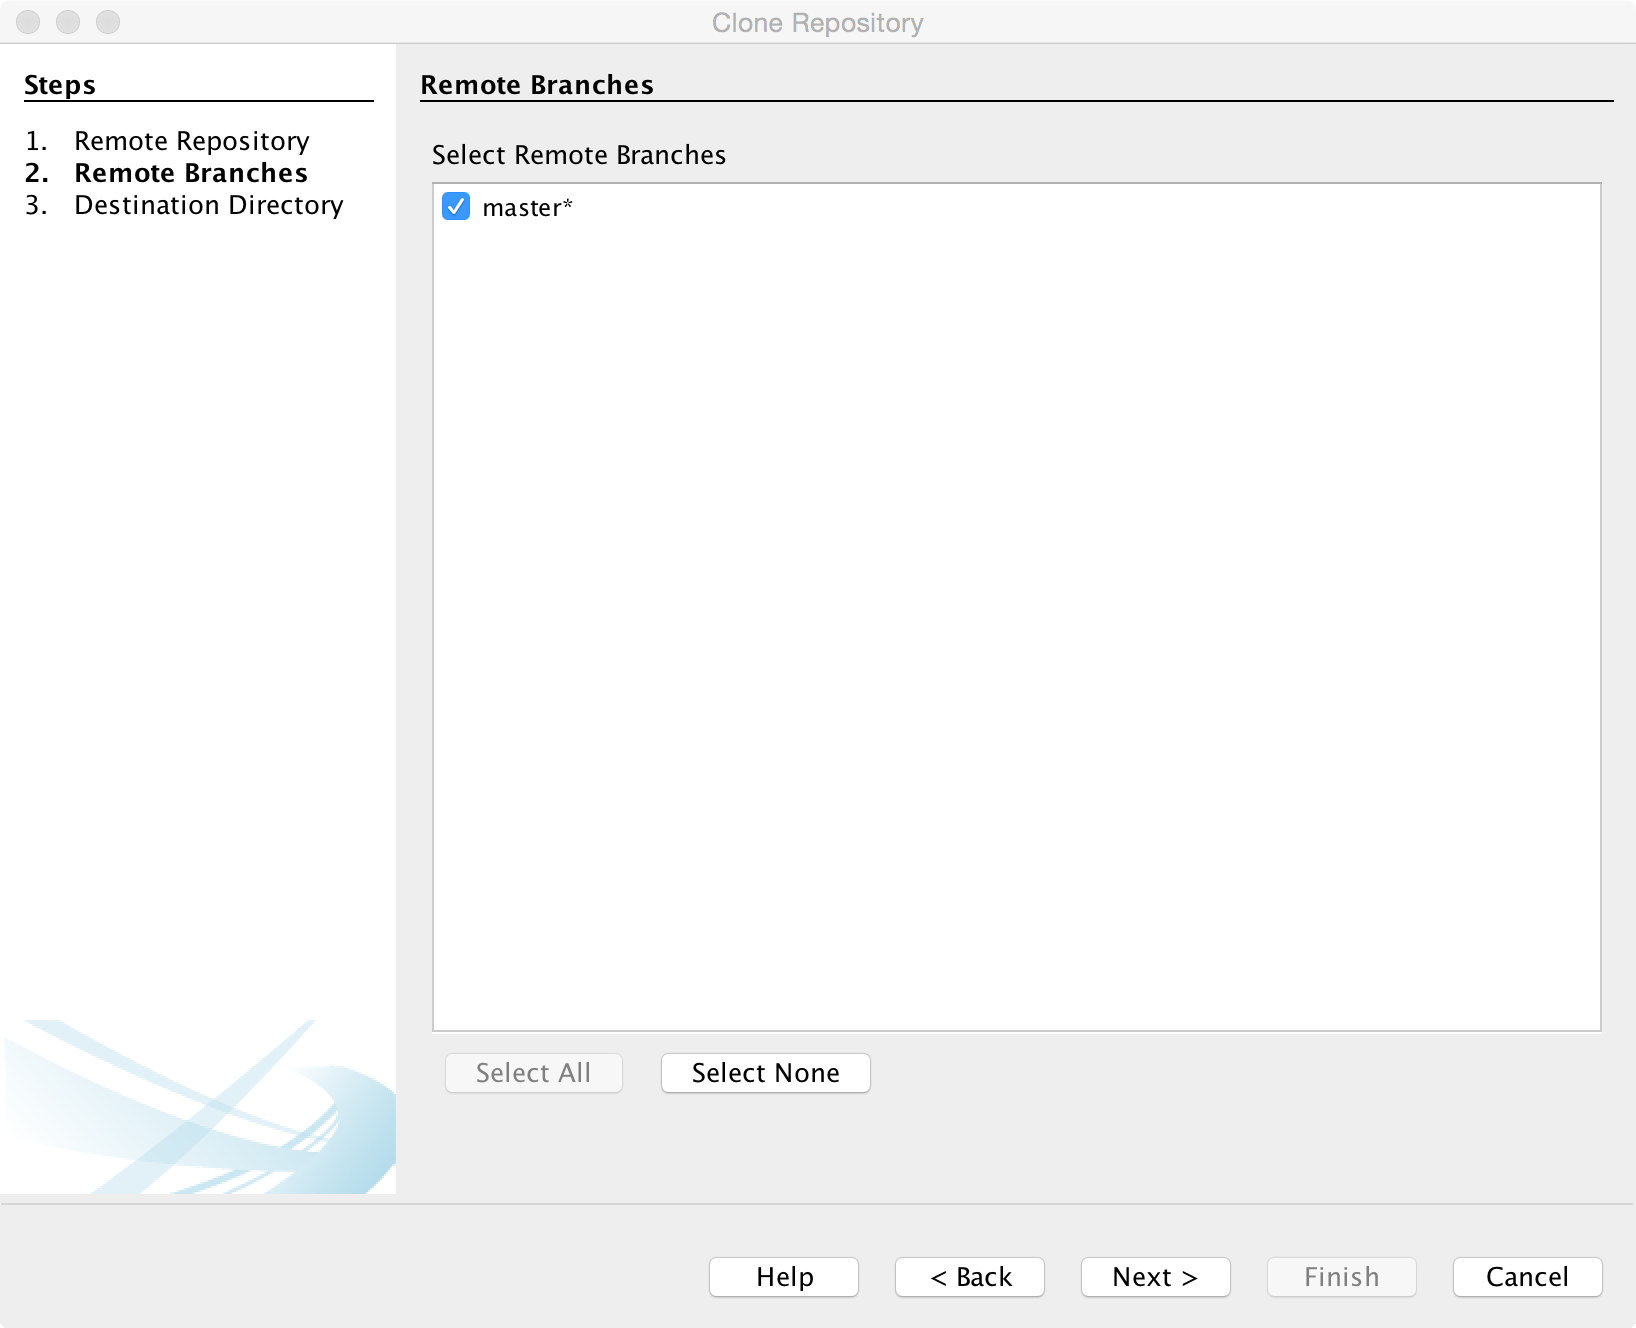
\includegraphics[width=.7\textwidth]{image/NetBeans_clone04.png}
			% \end{center}
		\item
			Dans \samp{Destination Directory} :
			de cliquer sur \samp{Finish} ;
		\item 
			Enfin, de confirmer l'ouverture du projet dans NetBeans
			\begin{center}
				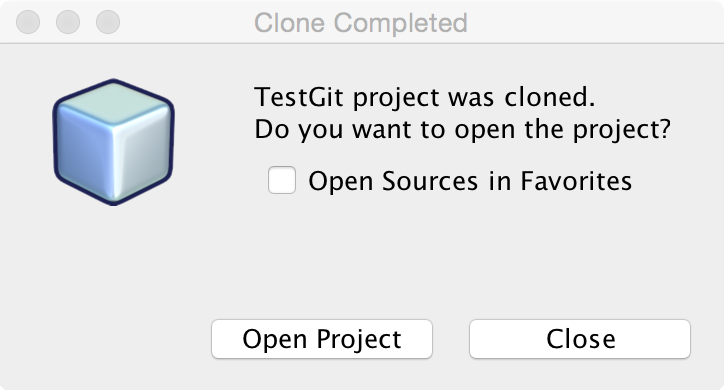
\includegraphics[width=.4\textwidth]{image/NetBeans_clone06.png}
			\end{center}			
		\end{steps}
	\end{steps}
\end{Tutoriel}
	
\begin{Tutoriel}{Continuer le projet}
	Continuons à développer le projet.
	Le programme doit désormais 
	afficher le nombre de caractères du nom encodé par l'utilisateur.
	Vous savez tout ce qu'il faut pour mener à bien cette tâche.
	\begin{steps}
		\item 
			Modifiez le programme ;
			\begin{center}
				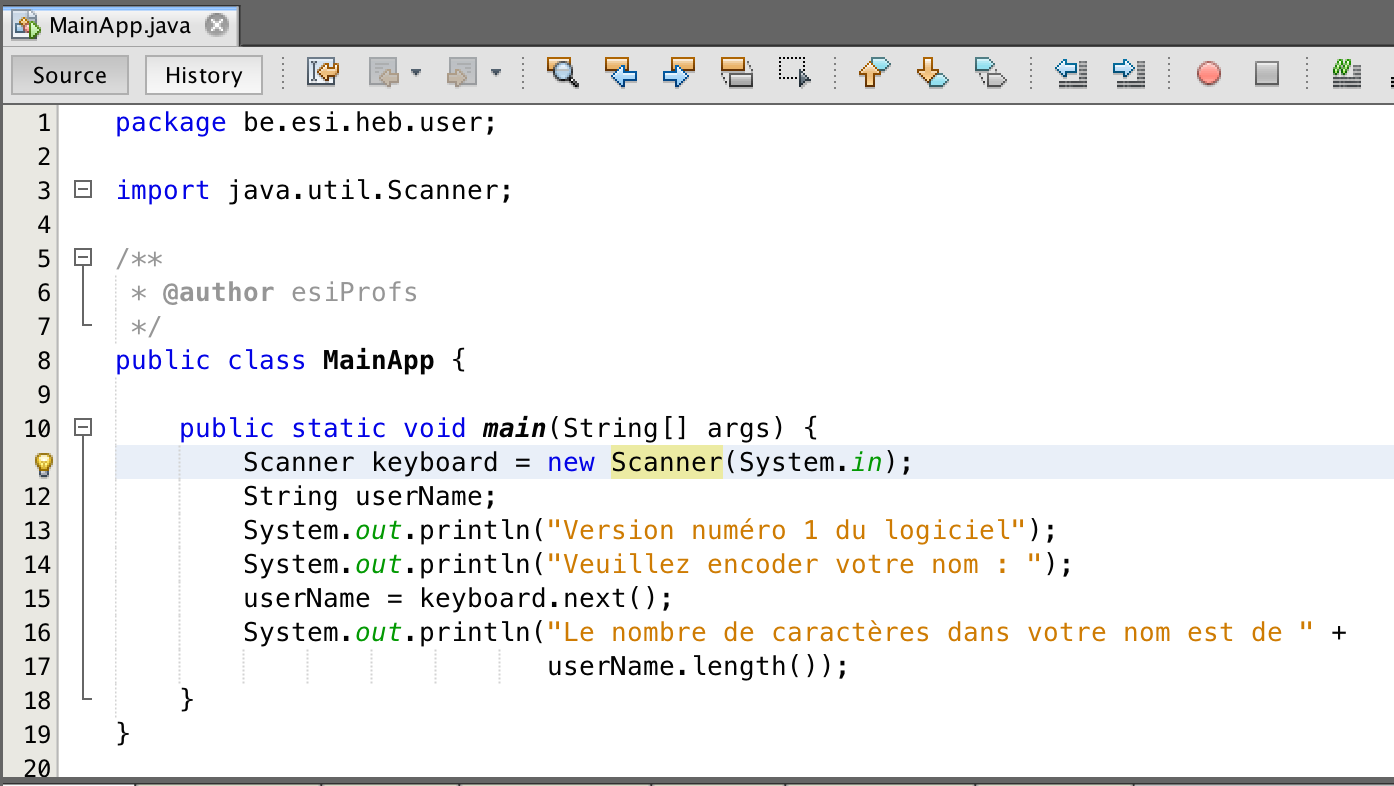
\includegraphics[width=.7\textwidth]{image/NetBeans_Project_10.png}
			\end{center}		
		\item 
			Effectuez un \textbf{commit} ;	
		\item 
			Effectuez un \textbf{push} ;
		\item 
			Allez sur le serveur et vérifiez que vos modifications s'y trouvent.
	\end{steps}
\end{Tutoriel}
	
%============================
\section{Reprendre un projet}
%============================

Voyons maintenant ce qui se passe lorsqu'on vous voulez reprendre
le travail sur la première machine.

Afin de continuer l'exercice déconnectez-vous de votre machine
et revenez à la machine du début du TD.

À tout de suite\dots{}

\begin{Tutoriel}{Pull}
	Vous voici de retour sur la machine du début.
	\begin{steps}
	\item 
		Ouvrez le projet \bsc{Netbeans}.
	\end{steps}
	Il est important de comprendre que cette version \textbf{n'est pas à jour}.

	\begin{infoit}{Pull}
		Un \textbf{pull}
		consiste à mettre à jour le contenu d'un dépôt.
		On va récupérer du serveur tous les commits manquants.
	\end{infoit}

	Pour récupérer les changements depuis le serveur,
	suivez les étapes ci-dessous.
	\begin{steps}
	\item 
		Dans l'onglet \samp{Projects} cliquez droit sur le projet.
	\item 
		Choisissez l'option \samp{Git > Remote > Pull...}.
	\end{steps}
	Par défaut, \bsc{Netbeans}
	entre en contact avec le serveur où vous avez effectué vos commits 
	et il récupére les nouveaux commits qu'il y trouve.
	\begin{steps}
	\item 
		Exécutez le projet, 
		vous constaterez qu'il s'agit bien de la version
		développée sur l'\textbf{autre} machine.
	\end{steps}
\end{Tutoriel}

%==================
\section{En résumé}
%==================

Voici un résumé des étapes par lesquelles vous devez passer
lorsque vous utilisez \bsc{git}.

\begin{infoit}{Démarrer un projet}
\begin{enumerate}
	\item Créez un projet sur le serveur%
		\footnote{Cette étape peut aussi se faire juste avant le push.} ;
	\item Créez un projet dans Netbeans ;
	\item Faites suivre le projet par git ;
	\item Faites un premier \textbf{commit} ;
	\item Faites un \textbf{push} pour le lier au projet sur le serveur
		et envoyer le premier commit.
\end{enumerate}
\end{infoit}

\begin{infoit}{Travailler sur un projet}
\begin{enumerate}
	\item 
		En début de séance vous \textbf{devez} faire 
		\begin{itemize}
		\item
			un \textbf{pull} 
				(si le projet existe déjà en local mais qu'il n'est pas à jour)
		\item 
			ou un \textbf{clone} (si le projet n'existe pas du tout sur cette machine).
		\end{itemize}
	\item Durant votre travail,
		dès que vous avez fini une fonctionnalité,
		vous \textbf{devez} faire un \textbf{commit}.
	\item 
		Après chaque commit ou une fois, en fin de séance,
		vous \textbf{devez} faire un \textbf{push}.
\end{enumerate}
\end{infoit}

\begin{alertit}{Erreur courante}
	Il est vraiment très important que vous soyez attentifs aux 2 points suivants :
	\begin{enumerate}
	\item 
		Avant de quitter votre poste de travail,
		faites un \textbf{commit} et un \textbf{push} de votre projet 
		afin que tout soit sur le serveur.
	\item
		Avant de continuer un projet,
		faite un \textbf{pull} afin de récupérer tout ce qui se trouve sur le serveur.
	\end{enumerate}
	Si vous ne suivez pas ces consignes,
	vous aurez des incohérences de dépôt qu'il sera plus difficile de corriger.
\end{alertit}

\newpage
%=================
\section{Exercice}
%=================

Nous vous proposons un seul exercice
consistant à déposer tous vos projets \bsc{Netbeans} développés
lors des précédents TDS sur gitlab afin de pouvoir en disposer partout.

\begin{infoit}{Limite sur les dépôts}
	L'administrateur du serveur \bsc{gitlab}
	a imposé une limite sur le nombre de dépôts que
	vous pouvez créer.
	C'est pourquoi nous vous recommandons de rassembler tout votre travail 
	actuel dans un seul projet \bsc{Netbeans}%
	\footnote{%
		Techniquement, 
		il est possible de déposer plusieurs projets \bsc{Netbeans}
		dans un même dépôt mais n'ajoutons pas de complexité
		dans le cadre de cette introduction à \bsc {git}.
	}
	si ce n'est pas encore fait.
\end{infoit}

%=================
\section{Conclusion}
%=================

\bsc{git} est un outil très puissant qui est devenu incontournable
dans le développement actuel.
Tout bon programmeur se doit de le connaitre.

Mais il est beaucoup plus riche que ce que vous venez d'en voir.
Un TD du laboratoire environnement sera entièrement consacré à \bsc{git}.
Il vous permettra d'apprendre à l'utiliser en mode commande
pour aller plus loin dans sa compréhension et ses possibilités.

\end{document}